% THIS IS SIGPROC-SP.TEX - VERSION 3.1
% WORKS WITH V3.2SP OF ACM_PROC_ARTICLE-SP.CLS
% APRIL 2009
%
% It is an example file showing how to use the 'acm_proc_article-sp.cls' V3.2SP
% LaTeX2e document class file for Conference Proceedings submissions.
% ----------------------------------------------------------------------------------------------------------------
% This .tex file (and associated .cls V3.2SP) *DOES NOT* produce:
%       1) The Permission Statement
%       2) The Conference (location) Info information
%       3) The Copyright Line with ACM data
%       4) Page numbering
% ---------------------------------------------------------------------------------------------------------------
% It is an example which *does* use the .bib file (from which the .bbl file
% is produced).
% REMEMBER HOWEVER: After having produced the .bbl file,
% and prior to final submission,
% you need to 'insert'  your .bbl file into your source .tex file so as to provide
% ONE 'self-contained' source file.
%
% Questions regarding SIGS should be sent to
% Adrienne Griscti ---> griscti@acm.org
%
% Questions/suggestions regarding the guidelines, .tex and .cls files, etc. to
% Gerald Murray ---> murray@hq.acm.org
%
% For tracking purposes - this is V3.1SP - APRIL 2009

\documentclass{acm_proc_article-sp}
\usepackage[none]{hyphenat}
\usepackage{ragged2e}
\usepackage{graphicx}
\usepackage{array}

\begin{document}

\title{Detecting and Combating ARP Spoofing}
%
% You need the command \numberofauthors to handle the 'placement
% and alignment' of the authors beneath the title.
%
% For aesthetic reasons, we recommend 'three authors at a time'
% i.e. three 'name/affiliation blocks' be placed beneath the title.
%
% NOTE: You are NOT restricted in how many 'rows' of
% "name/affiliations" may appear. We just ask that you restrict
% the number of 'columns' to three.
%
% Because of the available 'opening page real-estate'
% we ask you to refrain from putting more than six authors
% (two rows with three columns) beneath the article title.
% More than six makes the first-page appear very cluttered indeed.
%
% Use the \alignauthor commands to handle the names
% and affiliations for an 'aesthetic maximum' of six authors.
% Add names, affiliations, addresses for
% the seventh etc. author(s) as the argument for the
% \additionalauthors command.
% These 'additional authors' will be output/set for you
% without further effort on your part as the last section in
% the body of your article BEFORE References or any Appendices.

\numberofauthors{4} %  in this sample file, there are a *total*
% of EIGHT authors. SIX appear on the 'first-page' (for formatting
% reasons) and the remaining two appear in the \additionalauthors section.
%
\author{
% You can go ahead and credit any number of authors here,
% e.g. one 'row of three' or two rows (consisting of one row of three
% and a second row of one, two or three).
%
% The command \alignauthor (no curly braces needed) should
% precede each author name, affiliation/snail-mail address and
% e-mail address. Additionally, tag each line of
% affiliation/address with \affaddr, and tag the
% e-mail address with \email.
%
% 1st. author
\alignauthor
Chai Ming Xuan\\
       \affaddr{National University of Singapore}\\
       \email{mingxuan@u.nus.edu}
% 2nd. author
\alignauthor
Er Xue Hui\\
       \affaddr{National University of Singapore}\\
       \email{xuehuier@u.nus.edu}
% 3rd. author
\alignauthor 
Wu Wenqi\\
       \affaddr{National University of Singapore}\\
       \email{wenqi.wu@u.nus.edu}
\and  % use '\and' if you need 'another row' of author names
% 4th. author
\alignauthor Zhu Chunqi\\
       \affaddr{National University of Singapore}\\
       \email{chunqi@u.nus.edu}
}
\maketitle
\begin{abstract}
In light of the `Sparkle Vulnerability'\footnote{https://sparkle-project.org/documentation/security/} incident that occurred early in 2016, our team has been particularly interested in preventing Man-In-The-Middle (MITM) attacks, since that is one of its primary attack vectors. 

While internet security has generally increased over the past few years, there has been little improvements made to low-level protocols on the Link and Physical layers of the Open Systems Interconnection (OSI) model. Protocols such as Address Resolution Protocol (ARP) are still stateless, making them vulnerable to attacks. While solutions such as Secure ARP (S-ARP) exist, adoption of such solutions remain slow due to their incompatibility with existing protocols. The vulnerability in both ARP and DHCP makes carrying out MITM attacks via ARP spoofing or DHCP spoofing trivial. 

Thus, our research focuses on a solution to detect and prevent ARP and DHCP Spoofing while maintaining compatibility with existing protocols. This will greatly limit the MITM attack variants an attacker can consider. 

 
\end{abstract}

% A category with the (minimum) three required fields
\category{C.2.0}{Computer-Communication Networks}{General - Data Communications, Security and Protection}

%A category including the fourth, optional field follows...
\category{D.4.6}{Security and Protection}{Authentication,\\ Verification}

\terms{Network Security, Intrusion Detection System (IDS), \\
Address Resolution Protocol (ARP), spoofing \\ \\} 

\keywords{ARP spoofing, ARP Poisoning, network security, attack, MITM,
IDS, ARP protection\\} 

\section{Introduction}
The Address Resolution Protocol (ARP) is an important protocol in computer network communications. \\
In order for communication to occur between two computers, the computer will need to know two things - the IP and MAC address of the other computer. As IP addresses can be resolved using a DNS lookup, the ARP is used to determine the MAC address of the other computer given an IP address. Without the ARP, it would be difficult for computers to communicate with each other, as an IP-to-MAC address mapping needs to be established. 

Traditionally, the ARP cache has been an easy target for ARP attacks like ARP spoofing. Even until today, it is still relatively easy to carry out an ARP spoof, and it remains rather difficult to defend against it. 

There is a lack of viable solutions to protect the ARP cache because of the way it is designed. In fact, ARP spoofing is easy to carry out over a wireless network if it is not protected by WPA-Enterprise encryption. Over a Local Area Network (LAN), such attacks require a wiretap if the network uses switches instead of hubs. 

Some common attacks that can occur after an ARP Spoof are MITM, Denial-of-Service (DOS) and session hijacking. 
In such cases, the three basic principles of security -\\ Confidentiality, Integrity and Availability - may be violated. 
We will be illustrating how an ARP Spoof occurs in Section 2. 

Programs which users can use to carry out such an attack include but are not limited to, `Ettercap' and `Cain and Abel'. As these programs are open source and well documented, almost anyone can easily carry out ARP Spoofing with some basic technical knowledge. 

\newpage

\section{Background}
In order to understand how ARP spoofing occurs, we will need to cover the basics on how computers communicate with each other. In this section, we will be explaining how computers do so, and introduce the basic notions of how an ARP spoof is carried out. 

\subsection{Models and Abstractions}
In computer networking, the communication protocols are categorised and organised into different layers. There are 2 commonly used models - the TCP/IP model and the OSI model. 

In the TCP/IP Model, there are 5 layers of abstraction: 

1. Application Layer\\
2. Transport Layer\\
3. Network Layer\\
4. Link Layer\\
5. Physical Layer\\

DHCP is an application layer protocol and ARP is a link layer protocol.

In the OSI Model, there are 7 layers of abstraction:

7. Application Layer \\
6. Presentation Layer \\
5. Session Layer \\
4. Transport Layer \\
3. Network Layer \\
2. Data Link Layer \\
1. Physical Layer 

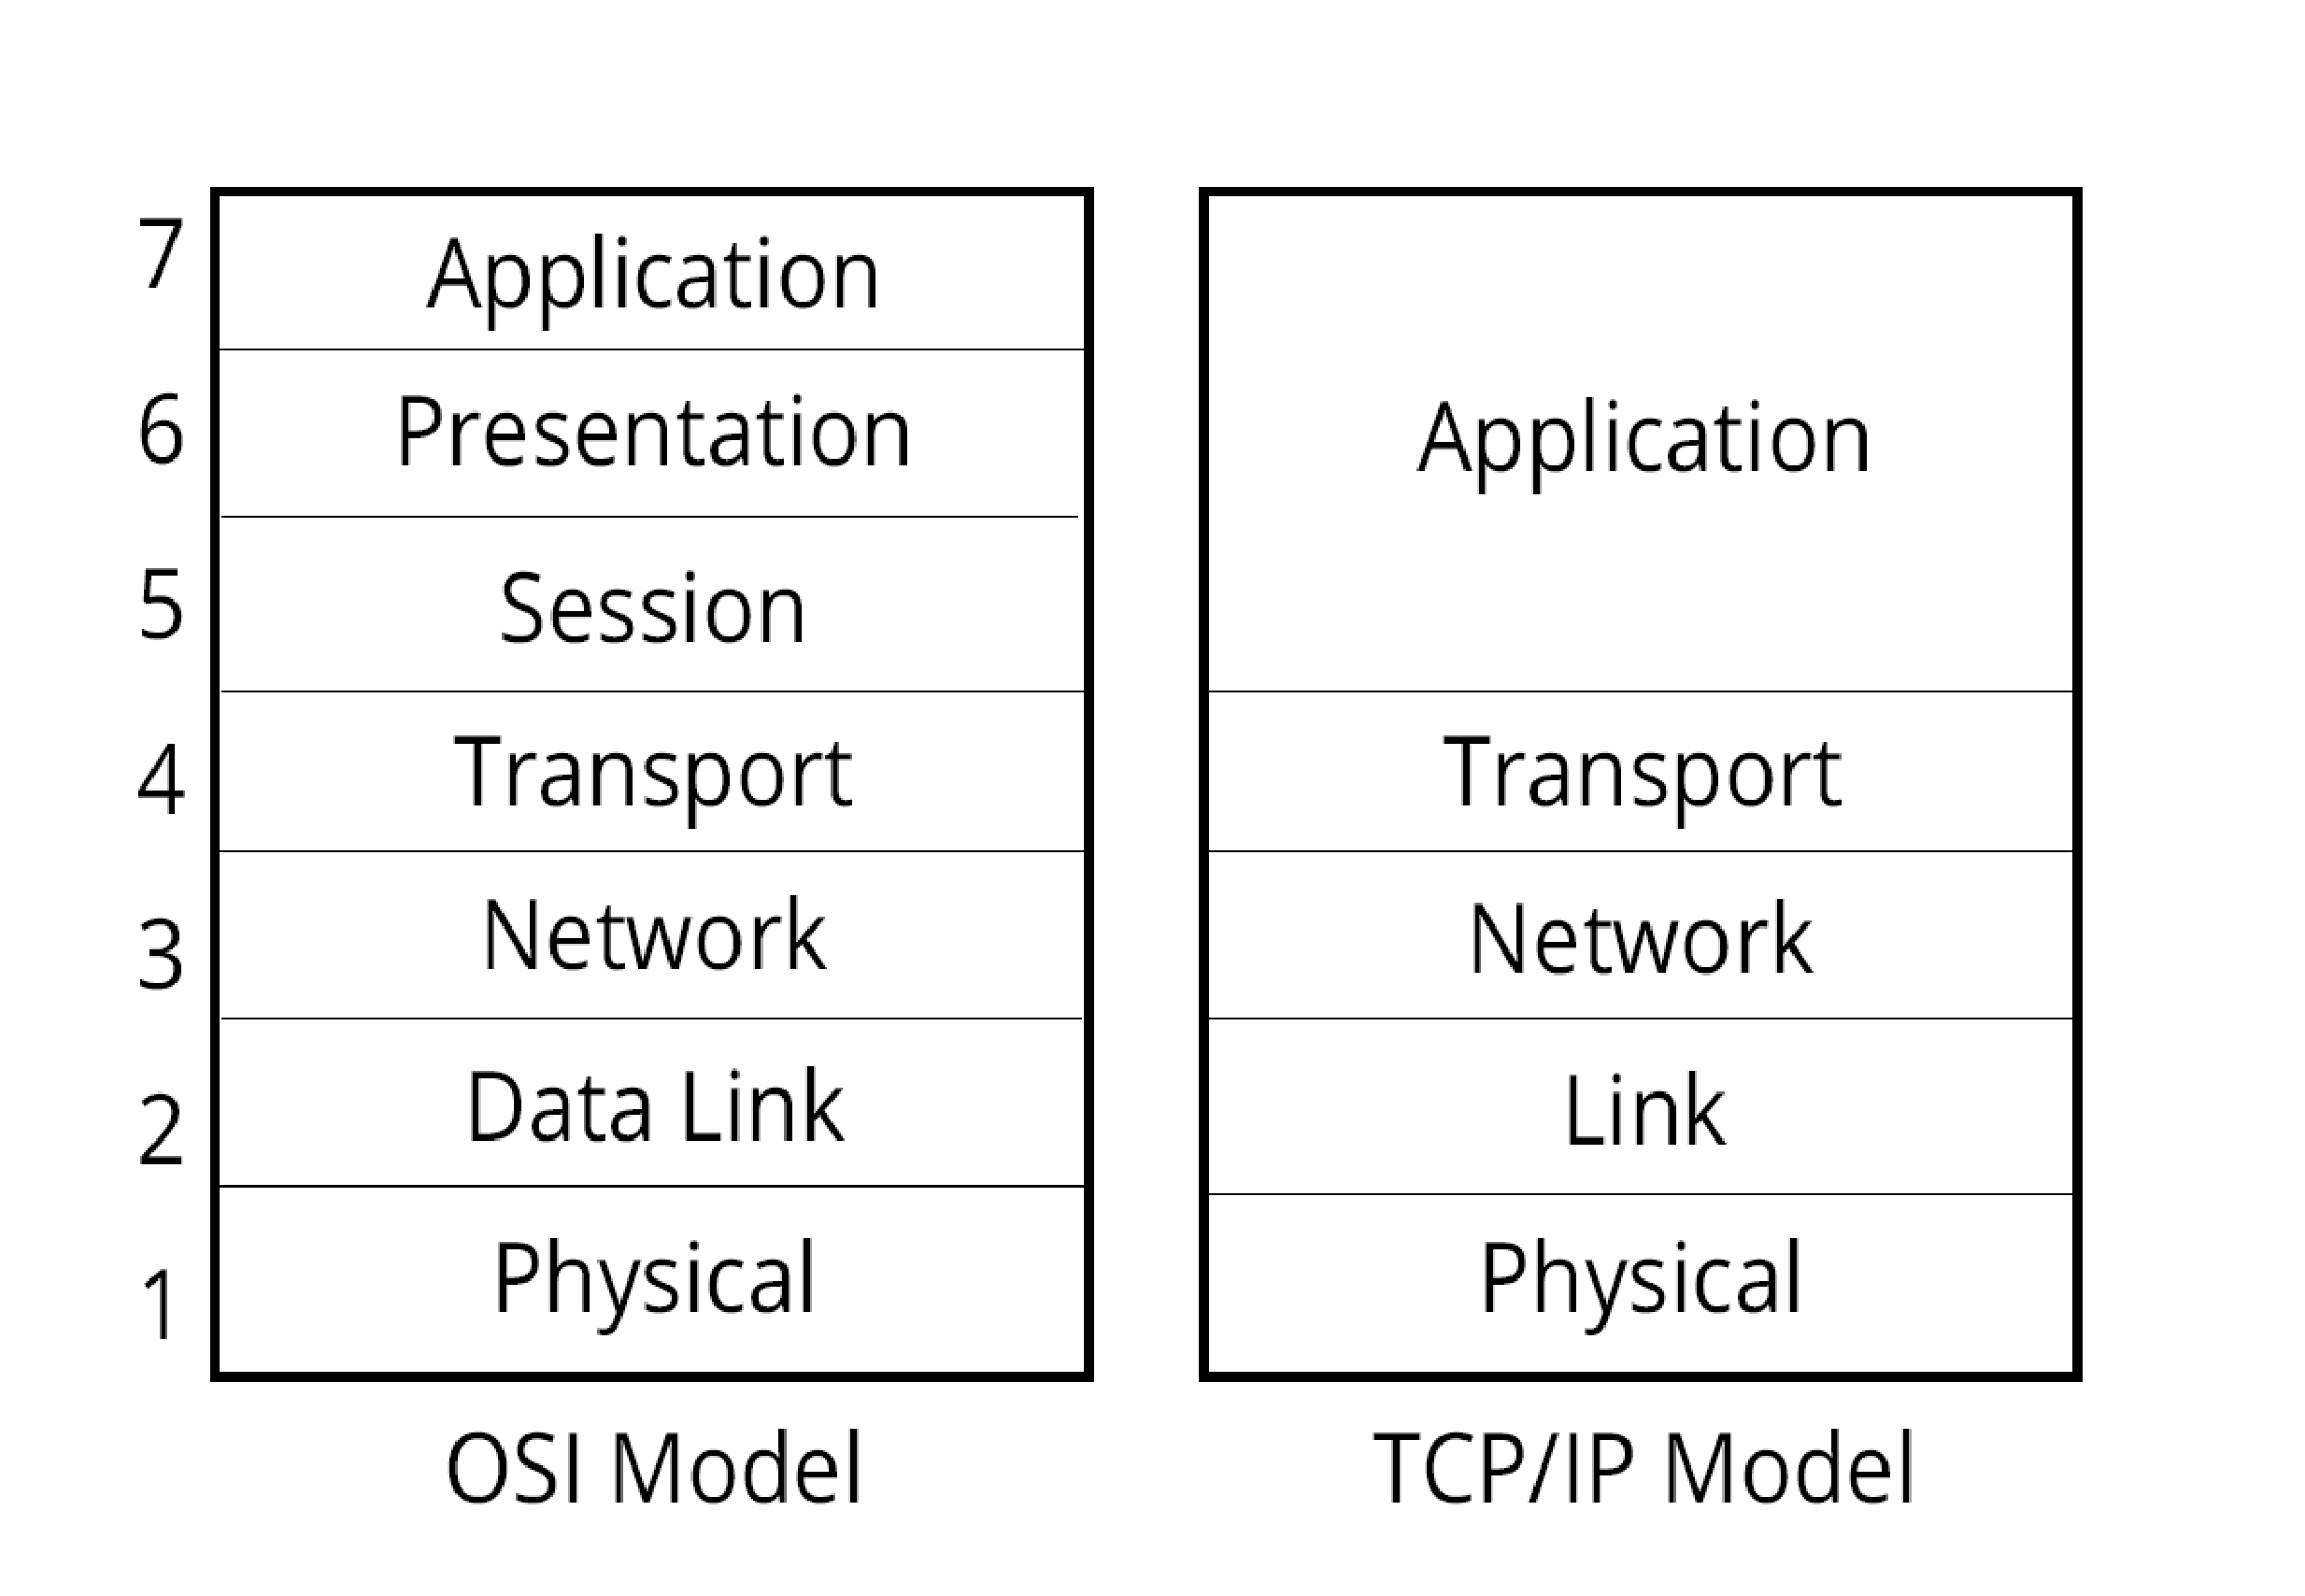
\includegraphics[width=2.7in]{osi_comparison.eps}

\subsection{Computer Communications}
In a typical modern computer, all IP addresses are resolved dynamically through the use of the Dynamic Host \\Configuration Protocol (DHCP). This is carried out in the following steps\cite{kurose:networking}: \\

1. DHCP Discover: \\
The new host broadcasts a DHCP discover message, where 255.255.255.255 is a typical broadcast address.  

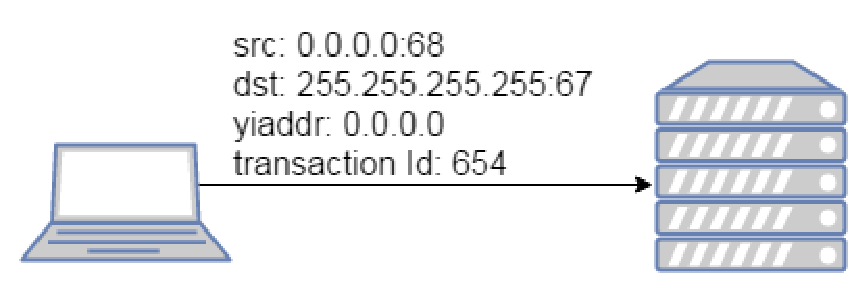
\includegraphics[width=3in]{DHCP_Discover.eps}

2. DHCP Offer: \\
The DHCP server responds with a DHCP offer. 

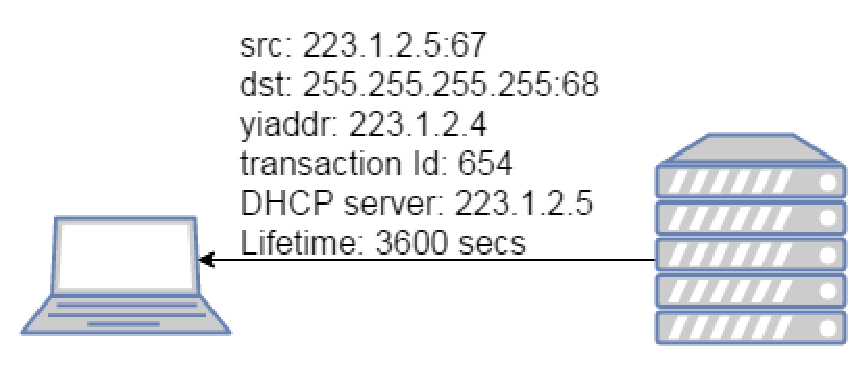
\includegraphics[width=3in]{DHCP_Offer.eps}

3. DHCP Request: \\
The host selects from the offers and sends a DHCP request. 

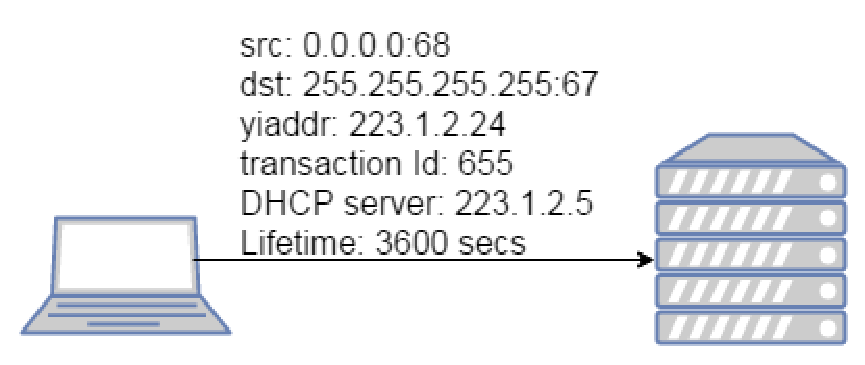
\includegraphics[width=3in]{DHCP_Request.eps}

4. DHCP ACK: \\ 
The DHCP Server confirms the requested parameters. 

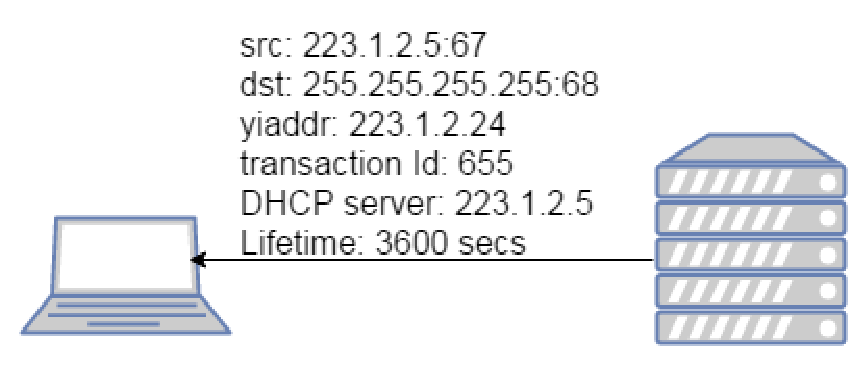
\includegraphics[width=3in]{DHCP_Ack.eps}

\newpage

After that, assuming everyone has already had their IPs assigned to them via DHCP, suppose the the user Alice wishes to send some information to Bob. The following steps are then carried out: 

1. ARP Request: Alice's computer sends out an ARP request to find out which MAC address has Bob's IP. 

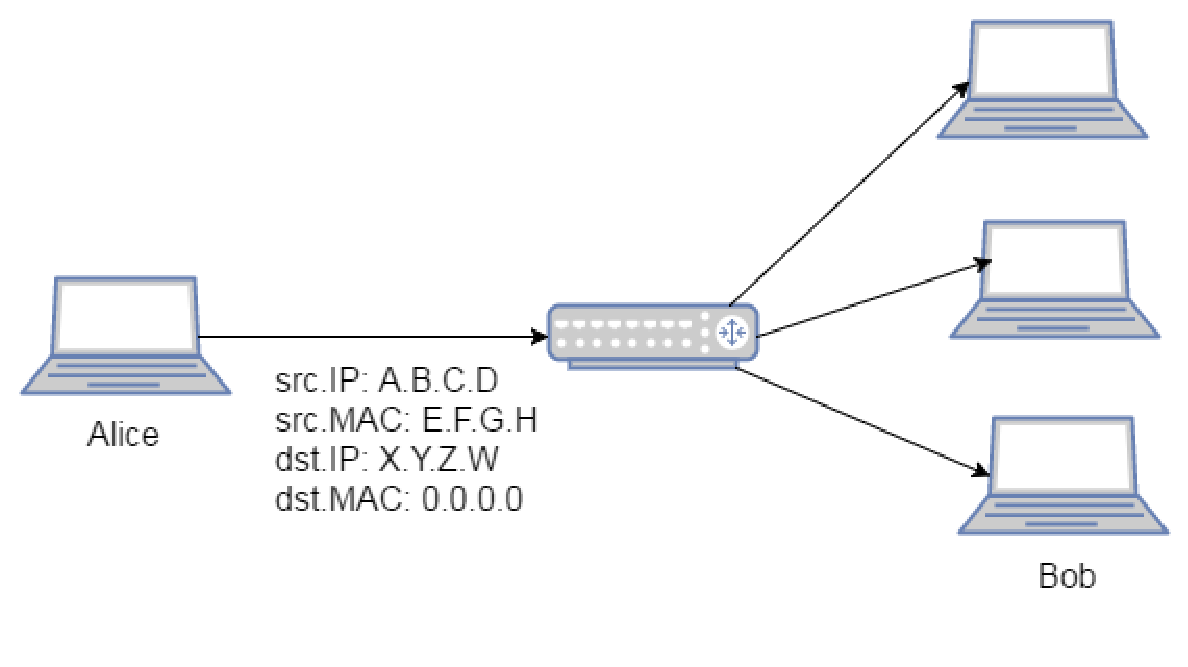
\includegraphics[width=3in]{ARP_Request.eps}

2. When Bob's computer receives the request, he sends back an ARP response packet. 

\includegraphics[width=3in]{ARP_Response.eps}

3. Alice gets the response and stores the corresponding IP-to-MAC entry into the ARP cache. 


\subsection{Poisoning the ARP Cache}
For ARP spoofing to work, the attacker typically has to be in the same network as his victim\cite{blackhat:arp5}. Sniffing is carried out to first determine the victim's IP address on the network. This can be done using a network sniffer such as Wireshark.  

There are 3 common ways to poison the ARP cache. The first is to send a broadcast request, the second is to send multiple responses, and the third is an unsolicited response. In this paper, we will only cover the second method\cite{wagner:arp4}.

If an attacker, Eve, wishes to carry out ARP spoofing, this is typically what happens: 

1. Alice's computer sends out an ARP request to find out what is Bob's MAC address. 

2. Before Bob's computer can reply, the attacker, Eve, sends a spam of packets to Alice's computer, claiming to be Bob. The ARP cache then becomes poisoned. 

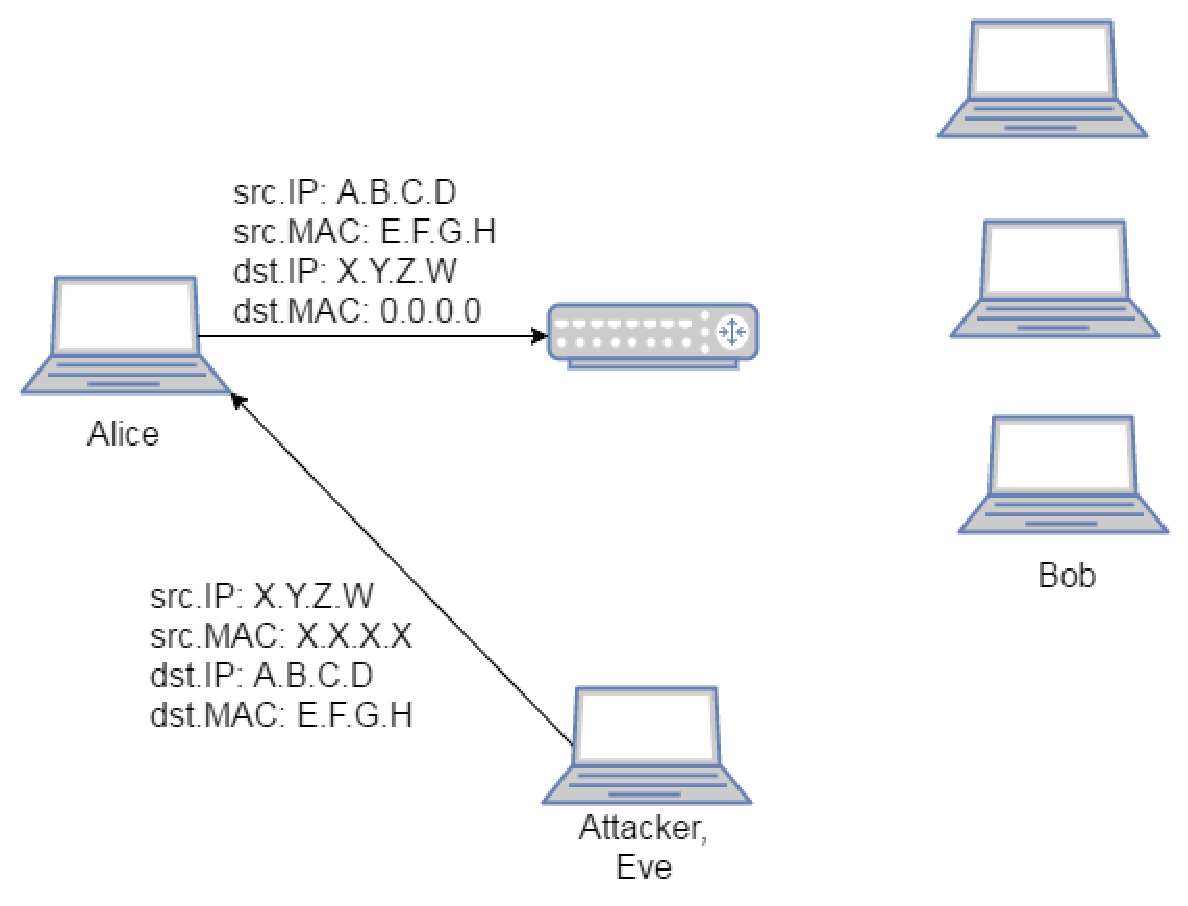
\includegraphics[width=3in]{Poisoned_ARP.eps}

In this case, there is a race condition between Eve and Bob to send a response to Alice. If Eve succeeds in responding to Alice before Bob can do so, Alice's ARP cache becomes successfully poisoned. 

\subsection{DHCP Spoofing}
In DHCP spoofing, there is a race condition between the rouge server and the legitimate server to respond to a user's DHCP Discover broadcast. 
Should the rouge server respond to the user first, the user then becomes subjected to an MITM attack. 

\includegraphics[width=3in]{DHCP_Spoofing.png}

The solution to this problem is to implement DHCP snooping. 

\section{Current Solutions and \\Mitigations}
There are currently many solutions in the market to combat ARP Spoofing. However, many of these solutions are described to have major issues. From \cite{vivek:arp}, \cite{navid:arp2} and \cite{goldendeep:arp3},  these are the summaries and drawbacks of current implementations in the market:

1. Use of Cryptographic Techniques \\
Examples: S-ARP \\
This method suggests that the ARP protocol be redesigned with cryptographic measures in place. However, implementing such cryptographic measures severely degrades the runtime performance of the ARP protocol. 

2. Passive Detection \\
Examples: Agnitum Outpost Firewall\\
Such methods only detect ARP spoofing but are unable to do anything to correct it. In addition, this method assumes that initial setting of ARP entries are correct, as the initial database is used for comparing with an incoming ARP packet to check if it has been spoofed. 

3. Kernel-based patches\\
Examples: Anticap, Antidote \\
A patch is given to fix the OS Kernel. However, this may cause compatibility issues. 

4. Making ARP entries static\\ 
In this method, ARP entries are configured to be static. In this case, DHCP will not be used to resolve local IP addresses for a computer. However, it will not be very user-friendly for standard office workers to configure, and will be very difficult for network administrators to manage IP-to-MAC mappings in a huge company. 


\section{Goals}
In taking up this project, we hoped to achieve the following goals: 

1. Provide users with a means to actively combat ARP spoofing \\
2. Make any network more secure. \\
3. Provide a GUI for users to see what is happening in their network in real-time. 

\section{Proof of Concept}
\subsection{Implementation System}
Operating System: \\
OSX El Capitan, Arch-Linux [Manjaro 15.12 Capella]

We created a software product called `Spoof Alert' to monitor the computer's network traffic and alert the user should there be any suspicious packets that hint at ARP or DHCP spoofing. Spoof Alert is implemented using Python 2.7 with scapy and tkinter as the main library dependencies.

\subsection{Assumptions}

There are many variants of ARP spoofing. In order to deliver a focused solution, we have made certain assumptions about our environment. Most of these assumptions are still likely hold in actual cases.

1. Attacker's computer has a normal network stack. 

2. All computers on the network have at least one TCP port open, since our solution requires computers to reply to TCP/SYN packets.

3. All computers on the network have a TCP/IP network stack up and running. 

4. The attacker will only ARP spoof an existing IP address. He will not spoof IP addresses which have not yet been issued by the DHCP server. 

5. At the start up of our application, the ARP cache of all computers are valid and no attacks should be taking place.


\subsection{Overall Architecture}
Spoof Alert's architecture shown in Figure 5.1. 

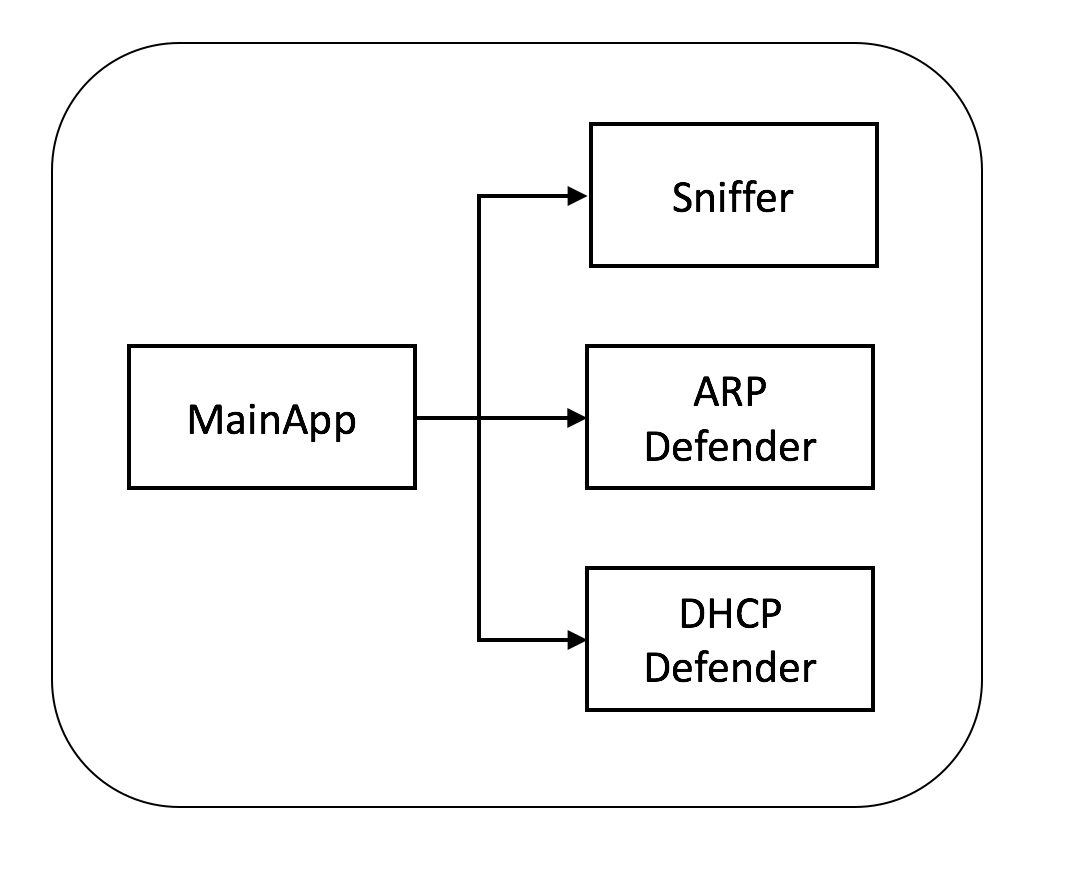
\includegraphics[width=3in]{architecture01.png} \\
Figure 5.1: High level view of Spoof Alert's architecture.

The sniffer runs on a separate thread from the main application and sniffs and filters out ARP and DHCP packets which are present in the network. Any packets the sniffer captures will be passed to a defender module (currently we have two such modules implemented), depending on the type of the packet. The defender module does a thorough inspection of any received packet (further elaborated in section 5.5). 

In future implementations, additional defender modules can be added to defend against a wider range of MITM attacks.

\subsection{The Attacker}

As we wanted to focus solely on developing the solution, we used Ettercap to test the performance of our software instead of writing our own attacker.  

\subsection{The Defender Module}

As of now, the ARP Defender and DHCP Defender modules have been implemented for Spoof Alert.

\subsubsection{ARP Defender module}

Upon receiving an ARP packet that is captured by the sniffer, the ARP Defender first checks that the packet's ARP header MAC and IP addresses for sender are consistent with that of its Ethernet headers. If there is a mismatch in headers, we conclude that the packet is invalid, and an ARP spoofing attack is potentially taking place.

If the headers match, we proceed to check if the packet is consistent with the entries in our ARP table, i.e. there is an entry in the ARP table which has the same sender IP and MAC addresses as the packet. If so, the packet is deemed to be a valid one, with the assumption that our ARP table has not been poisoned.

If the packet is inconsistent with the ARP table, Spoof Alert will perform an active check by sending a TCP SYN packet to the sender's IP address as stated in the packet. If there is a reply, we can assume the packet to be valid. Otherwise, it will be classified as a spoof packet.
A summary of the ARP defender’s process flow is shown in Figure 5.2.

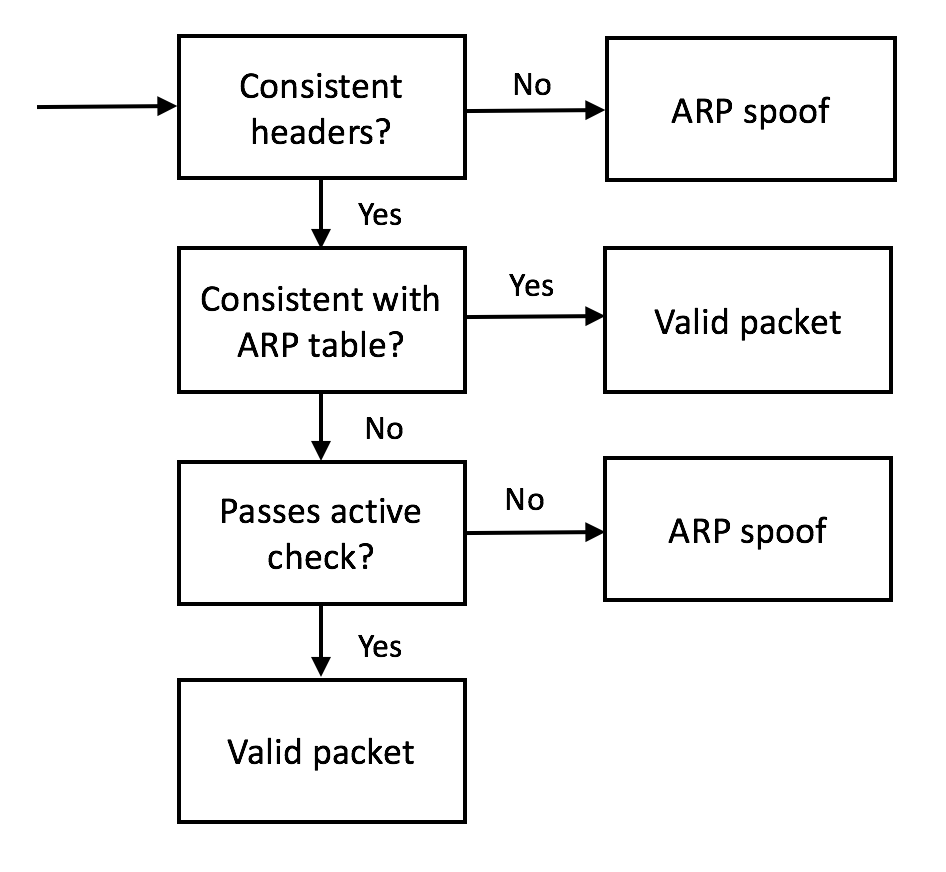
\includegraphics[width=3in]{architecture02.png} \\
Figure 5.2: Process flow of the ARP defender on receiving a packet.

\subsubsection{DHCP Defender module}

The DHCP Defender seeks to detect the presence of rogue DHCP servers in the network. While DHCP snooping allows the sending of DHCP offers by servers connected to a trusted port, this is only possible in a switched network. 

To allow detection of rogue servers in a wireless environment, Spoof Alert requires the valid DHCP servers in the network to have their IP and MAC address added its white-list. This requires the DHCP servers to have reserved static IP addresses in the network. Any computer that is not on the white-list but sends a DHCP offer will be treated as a rogue DHCP server. 

\subsection{The GUI}

Spoof Alert's view is split into several tabs. Below are some screenshots of our early prototype.

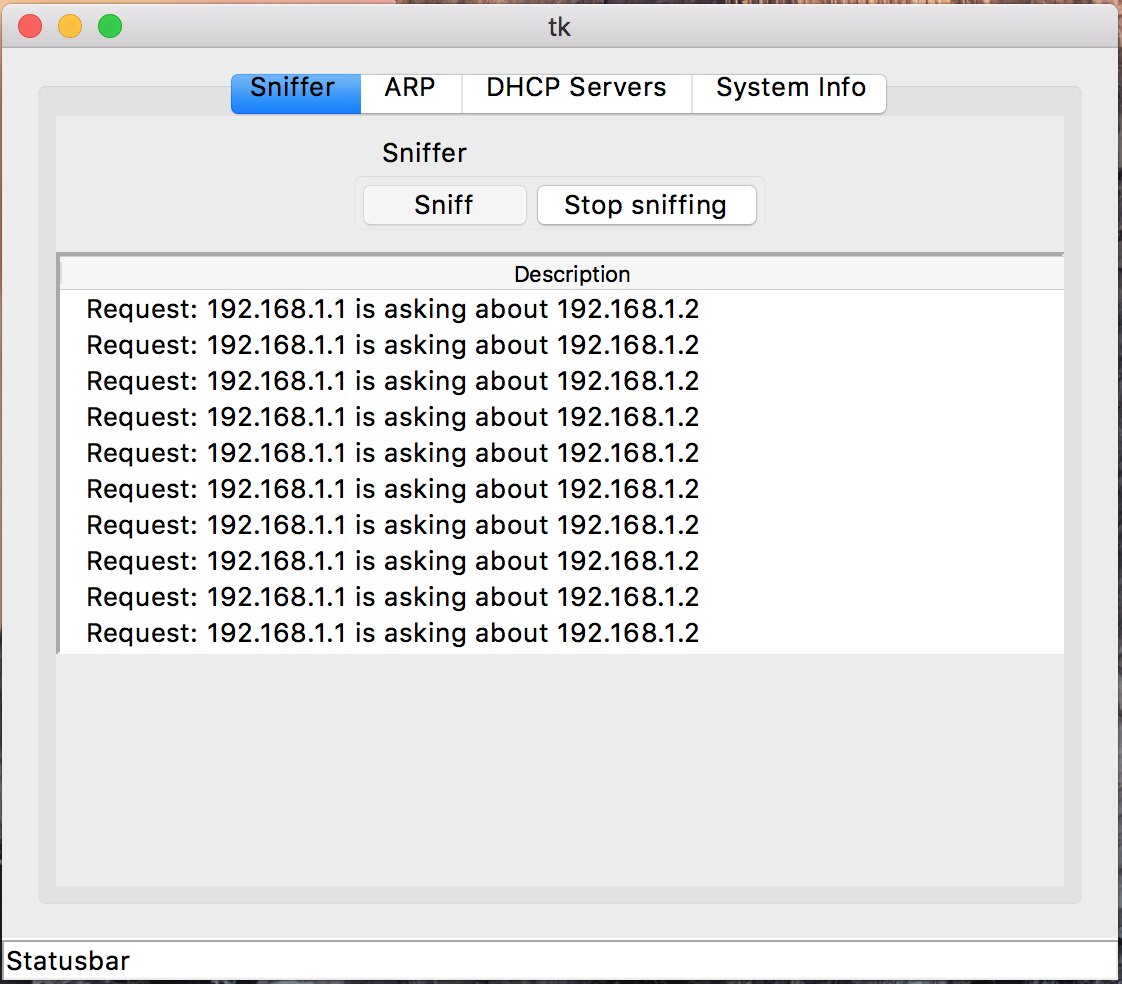
\includegraphics[width=3in]{architecture03.png} \\
Figure 5.3: In the Sniffer tab, the user can start the sniffer for Spoof Alert. All packets captured by the sniffer will be displayed here. Upon the detection of a suspicious packet, the user will be prompted by the application.

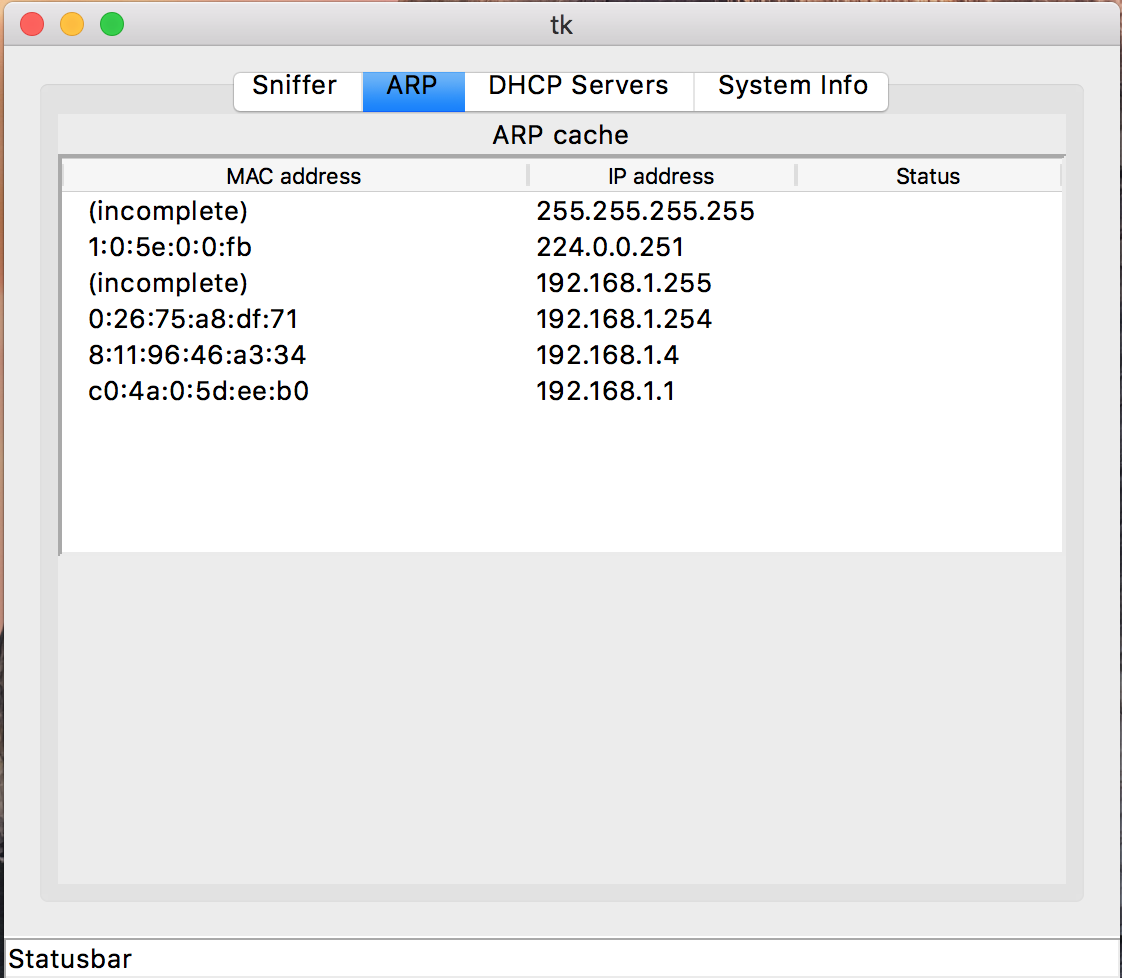
\includegraphics[width=3in]{architecture04.png} \\
Figure 5.4: In the ARP tab, the user can view the current entries in his computer’s ARP cache.

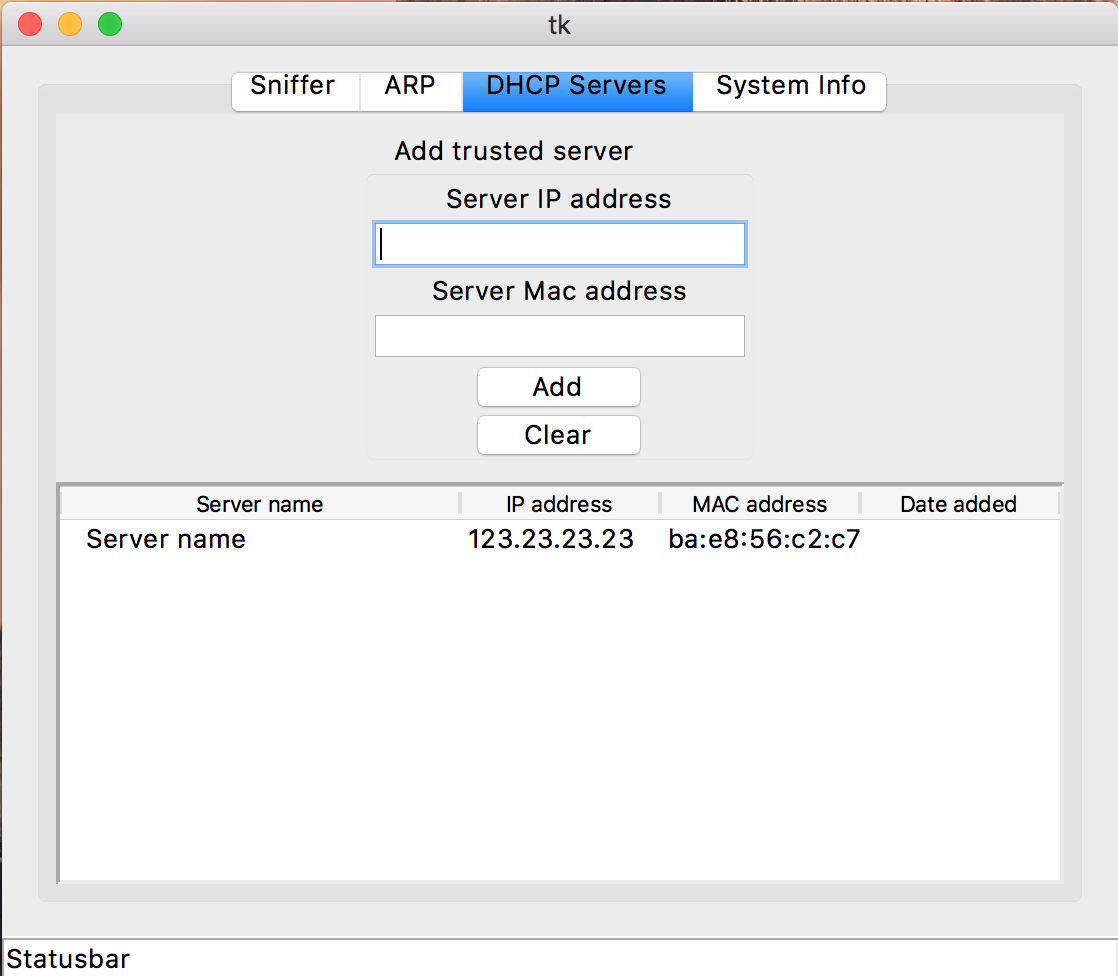
\includegraphics[width=3in]{architecture05.png} \\
Figure 5.5: In the DHCP servers tab, the user can add or remove DHCP servers from the white-list. If users wish to remove servers, they can only clear the entire list of servers. 

\section{Our solution versus current \\solutions}
In contrast to current available solutions, we tried to adopt an active method of detecting ARP spoofing, and avoid the weaknesses of current solutions.  

1. Secure ARP\\
Secure ARP (S-ARP) is an extension to the current ARP that allows authentication of ARP replies. However, this requires an additional header field to be added to the ARP packet and the network has to be modified to run authentication checks of S-ARP packets in order for this protocol to be supported. \\
Spoof Alert can be run from multiple client machines in the network and does not require any additional support.

2. arpwatch \\
arpwatch is a computer software tool used to monitor ARP packets in a network. Upon detecting that a MAC-IP address pairing has changed, arpwatch will send an email to the administrator as an alert to possible ARP spoof attack. This may result in false positives in an environment where IP addresses are assigned dynamically. \\
Upon detecting that a pairing has changed, Spoof Alert does not sound off the alarm immediately but sends a TCP SYN packet to the sender. If a response is given, it can be assumed that the packet is valid.

3. Static ARP \\ 
Static ARP will prevent all variants of ARP spoofing. However, this does not scale well in an large environment and gratuitous packets may not be supported by the network.

\section{Performance}
We tested the performance of our implementation using the Python library Scapy. The results are presented in Figure 7.1.

\begin{tabular}{ |m{15em}|m{7em}| }
\hline 
Experiment Parameters & Outcome \\
\hline 
 ARP response packet with inconsistent sender IP and MAC addresses in ARP and Ethernet headers & ARP spoof alert \\ 
\hline
 ARP response packet with consistent headers that is consistent with the ARP table &  Valid \\  
\hline
 ARP response packet with consistent headers that is inconsistent with the ARP table & ARP spoof alert \\
\hline
DHCP offer packet from white-listed computer & Valid \\
\hline
DHCP offer packet from non-white listed computer & DHCP spoof alert \\
\hline      
\end{tabular}


\section{Limitations and Future Work}
Our project has several issues which can be improved on.

\subsection{Limitations}
Currently, our tool only sniffs the network but does not prevent the addition of spoofed ARP pairings to the computer’s local ARP cache. If the attacker sets up a server on his attacking machine that responds to TCP SYN packets, it will bypass our detection system.

\subsection{Future Work: GUI}
1. A sleeker and more minimalistic UI will be implemented.

2. Support for removal of a single DHCP server entry from white-list.

3. Support the add-on of custom defender modules as well as allowing the user to control the packets to capture.

4. Come up with a less intrusive way of alerting the user of possible spoof attacks in the network.

5. Prevent the addition of spoofed ARP pairings to the computer’s local ARP cache

6. Various UI Bug fixes

\subsection{Future Work: Backend Code}

1. No Support for Network Encrypted with WPA-Enterprise:\\
Our solution will not work on a network that uses\\ WPA-Enterprise level of encryption. This is because the structure of WPA-Enterprise is such that each user can only see his incoming or outgoing network connections. 

2. Assumes the user is on an Insecure Network: \\
Our solution assumes that the user does not have any form of defence installed on his computer. (eg. no firewall that can prevent ARP spoofing, a network that does not use any enterprise level encryption, etc.) However, it is more likely that users have at least some kind of basic protection system on his computer. 

3. Tested Only on Wireless Networks:\\
The attacks have only been tested to work for various users across the wireless network which uses no encryption, WEP, WPA, and WPA2. While it might work on a network that uses a hub, it might require a wiretap for a switched network.  

We hope to improve our solution for a more varied set of systems in the future. Furthermore, if we are able to tell who our attacker is, we hope to implement a more aggressive method to counter their ARP attacks, such as spoofing them back. 

\section{Conclusion}
Through this project, we have learnt that ARP Spoofing is not easy to defend against. Even though there are solutions on the market that have been out for a while, unless one is using a network encrypted by WPA-Enterprise, it is otherwise easy to fall prey to such attacks. 

Furthermore, as active detection of ARP spoofing is not widely implemented yet, our solution may not be entirely foolproof. Thus, we will need to put in more work to make the solution more viable for a wider variety of situations. 

(to modify conclusion and include more stuff) 
%\end{document}  % This is where a 'short' article might terminate

%ACKNOWLEDGMENTS are optional
\section{Acknowledgements}
First and foremost, we would like to thank Prof. Hugh Anderson for his guidance and patience with us throughout the semester. Our initial project was to investigate the hacking of Hello Barbie. However, we eventually decided to change the topic for various reasons, and he very kindly allowed us to do so. This is despite the topic being changed quite late in the semester, and on top of it, was self-proposed. 

Our thanks also goes out to him for loaning us the Hello Barbie even though we eventually dropped the project. 

In addition, our appreciation also goes out to our friends who have given us technical advice, as well as loaned us various items for our project, such as a DLink Dir-825 router which runs on DD-RWT, so that we could work on the project in school. 

%
% The following two commands are all you need in the
% initial runs of your .tex file to
% produce the bibliography for the citations in your paper.
\bibliographystyle{abbrv}
\bibliography{sigproc}  % sigproc.bib is the name of the Bibliography in this case
% You must have a proper ".bib" file
%  and remember to run:
% latex bibtex latex latex
% to resolve all references
%
% ACM needs 'a single self-contained file'!
% 


\end{document}
